\documentclass[11pt,compress,xcolor=table]{beamer}

\usepackage[portuges]{babel}
\usepackage{lmodern}
\usepackage[utf8]{inputenc}

\usepackage{amssymb,amsmath}
\usepackage{amssymb}
\usepackage[T1]{fontenc}
\usepackage{textcomp}
\usepackage{verbatim}
\usepackage{bold-extra}
% pacote para colorir tabelas
\usepackage{color}
\usepackage{colortbl}
\usepackage{xcolor}
\usepackage[table]{xcolor}
%Colorir arquivos fontes
\usepackage{minted}
%caixas de textos
%\usepackage{fancybox}

%===== Pacotes para colorir links =====
\usepackage{fancyhdr}
%\usepackage[colorlinks,linkcolor=blue,hyperindex]{hyperref}
%\hypersetup{backref,  pdfpagemode=FullScreen, colorlinks=true,linkcolor=blue}

%===== Pacotes para mostrar códigos fontes =====
\usepackage{listings}
% simpsons
%\usepackage{simpsons}

% Caminhos das Imagens
\graphicspath{{images/}}

%cores
\definecolor{lightblue}{RGB}{0,159,253}

%comandos
\newcommand{\degree}{\ensuremath{^\circ}}
\makeatletter
  \newcommand\tinyv{\@setfontsize\tinyv{6pt}{6pt}}
\makeatother

%===== Configurações para mostrar Códigos Fonte ===== %
\lstset{numbers=left,
  language=python,
  stepnumber=1,
  firstnumber=1,
  numberstyle=\tiny,
  extendedchars=false,
  escapeinside='',
  breaklines=true,
  frame=tb,
  basicstyle=\tiny,
  stringstyle=\ttfamily,
  showstringspaces=false
  backgroundcolor=\icolor{gray}
  morecomment=[l]{//} % displays comments in italics (language dependent)
}

\author[Marczal, Kulk]{Diego Marczal \\ Josiel Neumann Kuk}
\title[Introdução ao Latex]{ Criando apresentações com o Beamer }
\subtitle[Apresentações]{{\scriptsize Porque formatações são chatas!!}}
\institute[UNICENTRO]{Universidade Estadual do Centro-Oeste}
\date[18/08/2011]{18 de agosto de 2011}

\logo{
\includegraphics[width=.5cm]{logo.jpeg}}

\usetheme{Ilmenau}
\setbeamercovered{transparent}
\setbeamertemplate{footline}[frame number]

\begin{document}


\begin{frame}
  \titlepage
\end{frame}

%-------------------------------------------------------------
%-------------------------------------------------------------

%================ Slide Sumario===============================
% cria o sumário
\begin{frame}[shrink,allowframeworks]
\frametitle{Sumário}
\tableofcontents[pausesections]
\end{frame}

%\begin{frame}[allowframeworks]
%\frametitle{Sumário}
%\tableofcontents[pausesections]
%\end{frame}

%------------------------------------------------------------
%============================================================

\section{Intro}

\subsection{O que é o Beamer}
%----------------------------------------------------------------------------%

\begin{frame}

  \begin{itemize}[<+->]
     \item Beamer é uma classe do \LaTeX para criar apresentações.
     \item Preparar apresentações com o Beamer é muito diferente do que utilizando
           os editores WYSIWYG, como o OpenOffice Impress, Apple Keynote, PowerPoint, etc..
     \item Uma apresentação Beamer é como qualquer outro documento do \LaTeX.
     \item Por isso, para usar o Beamer é necessário conhecer o \LaTeX.
  \end{itemize}

\end{frame}

%----------------------------------------------------------------------------%

\subsection{História}

\begin{frame}
   \begin{itemize}[<+->]
      \item Criado por \textbf{Till Tantau}.
      \item Till criou o Beamer para fazer a apresentação da Tese do seu Doutorado em 2003.
      \item Em 2010, \textbf{Joseph Wright e Vedran Miletić} passaram a manter o Beamer.
   \end{itemize}
\end{frame}

%----------------------------------------------------------------------------%
\section{Vantagens}
\subsection{Por que Utilizar Beamer?}

\begin{frame}
  \begin{itemize}[<+->]
     \item Os comandos padrões do \LaTeX também funcionam no Beamer.
     \item O sumário e as formações da apresentação são automaticamente criadas. Incluindo
          links para seção e subseção.
     \item É fácil criar animações e efeitos.
     \item Possui temas que permitem mudar aparência da sua apresentação com apenas um comando.
     \item Sendo cada tema desenvolvido para ser reutilizável em qualquer apresentação Beamer.
  \end{itemize}

\end{frame}

%----------------------------------------------------------------------------%

\begin{frame}
   \begin{itemize}[<+->]
      \item Os layouts, cores e as fontes podem ser facilmente alteradas tanto globalmente como
            localmente.
      \item É possível criar apresentações usando o mesmo código \LaTeX escrito para artigos.
      \item O saída gerada pela compilação dos códigos é geralmente no formato pdf.
      \item \alert{Sua apresentação terá \textbf{exatamente} mesmo formato em qualquer computador e SO!}
   \end{itemize}
\end{frame}

%----------------------------------------------------------------------------%

%Links
%  Página Inicial
%  Apoio (rails mg)
%  Sobre o evento
%  Programação
%  Palestrantes
%  Fale conosco
%     form
%     telefone
%     email
% Cadastro de emails
% Twitter
% FaceBook
% Orkut
% www.soeaa.com.br

\section{Templates}
\subsection{Como e por que Templates}

\begin{frame}
  \begin{itemize}[<+->]
     \item  O jeito mais rápido de começar com o Beamer é através do uso de templates.
     \item  Você pode gerar sua template através de scripts.
     \item  Vamos utilizar um \href{http:\\www.inf.ufpr.br/diego/minicurso\_latex}{\textcolor{blue}{script}}.
     \item  Crie uma basta \textbf{scripts} no seu home.
     \item  Descompacte os arquivos na pasta criada.
     \item  Execute o seguinte comando \textbf{./install}
  \end{itemize}
\end{frame}

\begin{frame}
  \frametitle{Teste o template}
  \begin{itemize}[<+->]
     \item Para criar uma apresentação execute o comando \textbf{latex\_new} nome da apresentação.
     \item Não use acentos nem espaços para a nome da apresentação.
     \item Para compilar entre no diretório do projeto e execute o comando \textbf{make}.
     \item Conhecendo a estrutura de diretórios e o arquivo \textbf{Makefile}.
  \end{itemize}
\end{frame}

\begin{frame}[fragile]
  \frametitle{Definindo informações}

    \only<1-5>{As primeiras alterações são para as informações chaves da sua apresentação}.

    \begin{block}{Alterações necessárias}<2->
      \begin{itemize}
         \item <2-> \mint{tex} |\title[Titulo menor]{Titulo maior}|
         \item <3-> \mint{tex} |\subtitle[Titulo menor]{Subtitulo maior}|
         \item <4-> \mint{tex} |\author[sobrenome]{nome}|
         \item <5-> \mint{tex} |\date[18/08/2011]{18 de agosto de 2011}|
     \end{itemize}
    \end{block}
\end{frame}

\section{Frames}
\subsection{Definindo slides}

\begin{frame}
  \frametitle{Frames}

  \visible<1-2>{Um projeto Beamer é constituído de vários \textbf{frames}. Cada \textbf{frame} produz um ou mais
  slides dependendo do uso dos \textit{overlays}.}

  \vspace{1cm}

  \begin{block}<2->{Examplo de um frame básico}
    \inputminted[fontsize=\scriptsize]{tex}{codes/01-frame.tex}
  \end{block}

\end{frame}

%-------------------------------------------------------------------------------------------------------------%

\begin{frame}

  \begin{block}<1->{Alinhamento}
    A opção de alinhamento \textit{default} é centralizada \textbf{[c]}.
    Mas existe as opções \textbf{[t]} para o alinhamento no topo (\textit{top align}), e \textbf{[b]} para
    o alinhamento no rodapé (\textit{bottom align}).
  \end{block}

  \vspace{1cm}

  \begin{block}<2>{Alinhamento}
    \inputminted[fontsize=\scriptsize]{tex}{codes/02-frame.tex}
  \end{block}
\end{frame}

%-------------------------------------------------------------------------------------------------------------%

\begin{frame}[plain]
  \begin{itemize}[<+->]
     \item A opção \textbf{plain} \textcolor{red}{$\backslash$begin\{frame\}[plain]}
           retira do slide os cabeçalhos, rodapés, e diminui a barra de navegação.
     \item Este recurso é importante para apresentar figuras.
  \end{itemize}
\end{frame}

%-------------------------------------------------------------------------------------------------------------%

\begin{frame}[fragile]
  \frametitle{Frames especiais}

  \begin{itemize}
     \item \mint{tex}|\titlepage|
     \item \mint{tex}|\tableofcontents[\pausesections] |
  \end{itemize}

   \begin{minted}[fontsize=\scriptsize,resetmargins=true]{tex}
     ..
     \begin{frame}
       \titlepage
     \end{frame}
     ...
     \begin{frame}
       \frametitle{Sumario}
       \tableofcontents
     \end{frame}
     ...
  \end{minted}

\end{frame}

%---------------------------------------------------------------------------------------%

\begin{frame}[fragile]
  \frametitle{Título do Frame}

   \begin{minted}[fontsize=\scriptsize,resetmargins=true]{tex}
     \begin{frame}
       \frametitle{Aqui vai o titulo do frame}
     \end{frame}
   \end{minted}

\end{frame}

%---------------------------------------------------------------------------------------%

\begin{frame}
  \frametitle{Tudo junto - Slides Iniciais}
  \inputminted[linenos,fontsize=\scriptsize]{tex}{codes/04-template-inicial.tex}
\end{frame}


\section{Seções}
\subsection{Particionando sua apresentação}

%--------------------------------------------------------------------------%

\begin{frame}[fragile]
  \begin{itemize}[<+->]
     \item Apresentações são divididas em seções, subseções, e sub-subseções.
     \item Para dividir sua apresentação utilize as instruções:
          \begin{minted}[fontsize=\scriptsize]{tex}
              \section{Titulo},
              \subsection{Titulo}
              \subsubsection{Titulo}
          \end{minted}
    \item \textcolor{red}{$\backslash$section\{...\}}
          \begin{itemize}
             \item Insere um novo tópico no sumário.
             \item Insere um novo \textit{link} na barra de menu.
             \item E não cria um cabeçalho no frame.
          \end{itemize}

     \item Outra versão:
          \begin{minted}[fontsize=\scriptsize]{tex}
            \subsection*{ ... }
          \end{minted}
          Apenas adiciona uma \textit{link} na barra de navegação, mas não no sumário.
   \end{itemize}
\end{frame}

%--------------------------------------------------------------------------%

\begin{frame}
  \frametitle{Exemplo}

  \inputminted[fontsize=\scriptsize]{tex}{codes/05-secoes.tex}

  Seções são sempre declaradas entre os frames!!!

\end{frame}



\section{Texto}
\subsection{Formatando Textos no Beamer}
%--------------------------------------------------------------------------%

\begin{frame}
  \frametitle{Comandos comuns para texto no Beamer}

  \begin{block}{}
      \begin{columns}
        \begin{column}[l]{5cm}
          \inputminted[fontsize=\small]{tex}{codes/06-text_commands.tex}
        \end{column}

        \begin{column}[c]{0cm}
          \line(0,0){100}
        \end{column}

        \begin{column}[r]{4cm}
          {\small
          \emph{Texto enfatizado}   \\
          \textbf{Texto em negrito} \\
          \textit{Texto em itálico} \\
          \textsl{Texto inclinado} \\
          \alert{Texto de alerta}  \\
          \textrm{Texto em romano} \\
          \textsf{Texto em sans serif} \\
          \textcolor{green}{Texto em verde} \\
          \texttt{Máquina de escrever} \\
          }
        \end{column}
      \end{columns}
  \end{block}

\end{frame}

%--------------------------------------------------------------------------%

\begin{frame}[fragile]
  \frametitle{Tamanho de Fontes}

  \begin{tabular}{|l|c|}
    \hline
      Comando & Resultado\\
    \hline
      \verb| \tiny{minúsculo} | & \tiny{minúsculo} \\
    \hline
      \verb| \scriptsize{muito pequena} | & \scriptsize{muito pequena} \\
    \hline
      \verb| \footnotesize{nota de rodapé} | & \footnotesize{nota de rodapé} \\
    \hline
      \verb| \small{pequena} | & \small{pequena} \\
    \hline
      \verb| \normalsize{normal} | & \normalsize{normal} \\
    \hline
      \verb| \large{grande} | & \large{grande}  \\
    \hline
      \verb| \LARGE{Muito Maior} | & \LARGE{Muito Maior} \\
    \hline
      \verb| \huge{Bem Grande} | & \huge{Bem Grande} \\
    \hline
      \verb| \Huge{Enorme} | & \Huge{Enorme}  \\
    \hline
  \end{tabular}

\end{frame}

%--------------------------------------------------------------------------%

\begin{frame}[fragile]
  \frametitle{Tamanho de Fontes}

  \rowcolors{1}{lightblue}{white}
  \begin{table}
    \begin{tabular}{|l|c|c|}
      \hline
        Comando & Tamanho - (padrão 12pt)\\
      \hline
        \verb| \tiny{minúsculo} | & 6pt\\
      \hline
        \verb| \scriptsize{muito pequena} | & 8pt\\
      \hline
        \verb| \footnotesize{nota de rodapé}| & 10pt\\
      \hline
        \verb| \small{pequena} | & 11pt\\
      \hline
        \verb| \normalsize{normal} | & 12pt \\
      \hline
        \verb| \large{grande} | & 17pt\\
      \hline
        \verb| \LARGE{Muito Maior} | & 20pt\\
      \hline
        \verb| \huge{Bem Grande} | & 25pt\\
      \hline
        \verb| \Huge{Enorme} | &  25pt\\
      \hline
    \end{tabular}
    \caption{Tamanho das fontes}
    \label{Tamanho das fontes}
  \end{table}

\end{frame}

%--------------------------------------------------------------------------%

\begin{frame}[fragile]
  \frametitle{Texto Verbatim}

  \begin{itemize}[<+->]
     \item Em alguns momentos necessitamos digitar algum texto do jeito que escrevemos.
     \item Mas como fazer isto no \LaTeX?
     \item No \LaTeX uma das maneiras é utilizar o comando \textbf{verbatim}.
  \end{itemize}

  \vspace{1cm}
  \visible<4>{Existe duas maneiras de usar o \textbf{verbatim}:}

\end{frame}

%--------------------------------------------------------------------------%

\begin{frame}[fragile]
  \frametitle{Usando texto verbatim}

  \begin{itemize}[<+->]
     \item Para textos de uma linha usa-se: \\
        \begin{minted}[fontsize=\scriptsize, resetmargins=true]{tex}
            \verb|Qualquer texto...|
        \end{minted}
     \item Para grande quantidades de textos:
        \begin{minted}[fontsize=\scriptsize, resetmargins=true]{tex}
          \begin{verbatim}
             Texto ...
             Texto ...
             .....
          \end{verbatim}
        \end{minted}
  \end{itemize}

  \begin{block}<3->{Nota:}
    Para o \textbf{verbatim} funcionar é necessário adicionar a opção [fragile] no frame.
    Exemplo: \mint{tex}| \begin{frame}[fragile] ...|
  \end{block}

\end{frame}

%--------------------------------------------------------------------------%

\begin{frame}[fragile]
  \frametitle{SemiVerbatim}

  \begin{block}<1->{Exemplo de código:}
     \begin{minted}[fontsize=\scriptsize, resetmargins=true]{tex}
        \begin{semiverbatim}
           Para o texto em vermelho use o comando
           \textcolor{red}{ \\textcolor\{red\}\{Vermelho\} }
        \end{semiverbatim}
     \end{minted}
  \end{block}

  \begin{block}<2->{Resultado:}
    \begin{semiverbatim}
      Para o texto em vermelho use o comando
      \textcolor{red}{ \\textcolor\{red\}\{Vermelho\}}
    \end{semiverbatim}
  \end{block}
\end{frame}

%--------------------------------------------------------------------------%

\begin{frame}[fragile]
  \frametitle{Temas de Fonte}
  \begin{itemize}
     \item<1-> Para mudar o tipo de fonte da apresentação usamos o comando:
        \mint{tex}| \usefonttheme{serif}|
  \end{itemize}

  \begin{block}<2->{Você pode escolher as seguintes opções de temas:}
    \begin{center}
       \begin{tabular}{ll}
        serif & structureitalicserif \\
        structurebold & structuresmallcapsserif
      \end{tabular}
     \end{center}
  \end{block}

  \begin{block}<3->{Nota:}
    Para mais informações sobre fontes \textbf{leia o Beamer User Guide}
  \end{block}

\end{frame}

%--------------------------------------------------------------------------%
\begin{frame}[fragile]
  \frametitle{Tamanho de Fonte}
  \begin{itemize}
     \item Para escolher o tamanho da fonte é necessário adicionar parâmetros no inicio do documento Beamer.
        \mint{tex}|\documentclass{beamer}|
     \item Exemplo:
        \mint{tex}|\documentclass[10pt]{beamer}|
     \item As opções de tamanho são:
          \begin{itemize}
             \item 10pt
             \item 11pt (Tamanho padrão)
             \item 12pt
          \end{itemize}
     \item Outras tamanhos requerer o uso de pacotes adicionais!
  \end{itemize}

\end{frame}

%--------------------------------------------------------------------------%

\begin{frame}[fragile]

  \frametitle{Definindo novo tamanho de fonte}

  Para definir um tamanho de fonte precisa-se criar um comando!

  \begin{block}<1->{}
     \begin{minted}[fontsize=\scriptsize, resetmargins=true]{tex}
       \makeatletter
         \newcommand\tinyv{\@setfontsize\tinyv{6pt}{6pt}}
       \makeatother
     \end{minted}
  \end{block}

  \begin{block}<2->{Exemplo:}
    \begin{columns}
      \begin{column}[l]{5cm}
         \mint{tex}| \tinyv{Fonte ainda menor} |
      \end{column}

      \begin{column}[r]{0cm}
         $\rightarrow$
      \end{column}

      \begin{column}[r]{4cm}
        \tinyv{Fonte ainda menor}
      \end{column}
    \end{columns}
  \end{block}

\end{frame}

%--------------------------------------------------------------------------%

\begin{frame}[fragile]
  \frametitle{Estilos de Fonte}

  Diferentes estilos de fontes podem ser escolhidos para personalizar sua apresentação. \\

  Cada estilo de fonte está separada em um pacote diferente.
  \mint{tex}|\usepackage{helvet}|

  Para usar um estilo def fonte use o comando:
  \mint{tex}|\fontfamily{euler}|

  \begin{block}{Fontes disponíveis no Beamer}
    \begin{tabular}{l l l l l}
      serif & euler & newcent & avant & helvet \\
      palatino & bookman & mathtime & pifont & chancery \\
      mathptm & utopia & charter & mathptmx \\
    \end{tabular}
  \end{block}

\end{frame}

\section{Posições}
\subsection{Alinhamento e Espaçamento}
%-----------------------------------------------------------------%

\begin{frame}[fragile]
  \frametitle{Alinhamento}

  Um frame pode ser alinhado a \textbf{esquerda}, \textbf{direita} ou \textbf{centro} com os
  seguintes comandos
  \begin{itemize}
     \item \mint{tex}|\flushleft{Texto}|
     \item \mint{tex}|\flushright{Texto}|
     \item \mint{tex}|\center{Texto}|
  \end{itemize}

  \begin{block}{Exemplo:}
    \begin{columns}
      \begin{column}[l]{5cm}
        \begin{minted}[fontsize=\scriptsize,resetmargins=true]{tex}
          \begin{center}
            Texto Centralizado
          \end{center}
        \end{minted}
      \end{column}

      \begin{column}[r]{5cm}
          \begin{center}
            Texto Centralizado
          \end{center}
      \end{column}
    \end{columns}
  \end{block}

\end{frame}

%-----------------------------------------------------------------%
\begin{frame}[fragile]

  \begin{block}<1->{Código para alinhar a esquerda}
    \mint{tex}| \flushleft{A esquerda} |
  \end{block}

  \begin{block}<2->{Resultado:}
     \flushleft{A esquerda}
   \end{block}

  \begin{block}<3->{Código para alinhar a direita}
    \mint{tex}| \flushright{A direita} |
  \end{block}

  \begin{block}<4->{Resultado:}
     \flushright{A Direita}
  \end{block}

\end{frame}

%-----------------------------------------------------------------%

\begin{frame}[fragile]
  \frametitle{Espaçamento}

  \begin{itemize}[<+->]
     \item O espaço vertical é indicado usando o comando \textcolor{green}{$\backslash$vskip<number>pt}. \\
           Por exemplo: \textcolor{green}{$\backslash$vskip15pt} irá produzir 15 pontos de espaço na vertical.
     \item O mesmo acontece para o espaço horizontal:
           Por exemplo: \textcolor{green}{$\backslash$hskip15pt}| irá produzir 15 pontos de espaço na horizontal.
     \item Espaços horizontais são úteis para indentar textos ou gráficos.
     \item Também é possível usar medidas em \textbf{cm}. \\
           Exemplo: \textcolor{green}{$\backslash$vskip15cm}
     \item Valores negativos também sào permitidos.\\
           Exemplo: \textcolor{green}{$\backslash$vskip-10pt ou $\backslash$hskip-1cm}
  \end{itemize}

\end{frame}

%-----------------------------------------------------------------%

\begin{frame}
  \frametitle{Espaçamento}
  Ainda temos os comandos:
  \begin{itemize}[<+->]
     \item \textbf{$\backslash$vspace\{<numero>pt\}}
     \item \textbf{$\backslash$hspace\{<numero>pt\}}
     \item Também podem ser usados em \textbf{cm}
  \end{itemize}

\end{frame}


%%!TEX encoding = UTF-8 Unicode
\section{Listas}
\subsection{Definindo Listas}
%-----------------------------------------------------------------%

\begin{frame}

  Lista são frequentemente utilizados para organizar os assuntos apresentação em tópicos. \\

  O Beamer inclui três formas de organizar sua apresentação em tópicos. \\

  \begin{description}
     \item[\textbf{Itemize}] Usado para apresentar uma lista de itens que não possuem uma ordem.
     \item[\textbf{Enumerate}] Usado para mostrar uma lista com números (itens ordenados).
     \item[\textbf{Description}] Usado para mostrar itens com explicações.
  \end{description}

\end{frame}

%-----------------------------------------------------------------%

\begin{frame}[fragile]
  \frametitle{Itemize}

  \begin{columns}
    \begin{column}[l]{5cm}
     \begin{minted}[fontsize=\scriptsize, resetmargins=true]{tex}
      \begin{itemize}
         \item Primeiro Item.
         \item Segundo Item.
         \item Terceiro Item.
         \item Quarto Item.
      \end{itemize}
  \end{minted}

    \end{column}

    \begin{column}[r]{5cm}
      \begin{itemize}
         \item Primeiro Item.
         \item Segundo Item.
         \item Terceiro Item.
         \item Quarto Item.
      \end{itemize}
    \end{column}
  \end{columns}
\end{frame}

%-----------------------------------------------------------------%

\begin{frame}[fragile]
  \frametitle{Enumerate}

  \begin{columns}
    \begin{column}[l]{5cm}
     \begin{minted}[fontsize=\scriptsize, resetmargins=true]{tex}
      \begin{enumerate}
         \item Primeiro Item.
         \item Segundo Item.
         \item Terceiro Item.
         \item Quarto Item.
      \end{enumerate}
  \end{minted}

    \end{column}

    \begin{column}[r]{5cm}
      \begin{enumerate}
         \item Primeiro Item.
         \item Segundo Item.
         \item Terceiro Item.
         \item Quarto Item.
      \end{enumerate}
    \end{column}
  \end{columns}
\end{frame}

%-----------------------------------------------------------------%

\begin{frame}[fragile]
  \frametitle{Description}

    \begin{block}{}
      \inputminted[fontsize=\scriptsize]{tex}{codes/07-description.tex}
    \end{block}

    \begin{block}{}
       \begin{description}[Primeiro Item]
          \item [Primeiro Item] Descrição do primeiro item.
          \item [Segundo Item] Descrição do segundo item.
          \item [Terceiro Item] Descrição do terceiro item.
          \item [Quarto Item]  Descrição do quarto item.
       \end{description}
   \end{block}

\end{frame}


%-----------------------------------------------------------------%

\section{Overlays}
\subsection{Criando efeitos no texto}

%-----------------------------------------------------------------------%

\begin{frame}
  \frametitle{Overlays}

  \begin{itemize}[<+->]
     \item São usado para partes da apresentação aparecerem incrementalmente.
     \item No Beamer, os \textcolor{red}{overlays} controlam que partes do frame irá aparecer.
  \end{itemize}

\end{frame}

%-----------------------------------------------------------------------%

\begin{frame}[fragile]
  \frametitle{Overlays}

  \begin{block}<1->{}
    Uma das maneiras de fazer partes dos texto aparecerem separados é utilizando o comando
    \mint{tex}| \pause |
  \end{block}

  \begin{block}<2->{Exemplo do pause:}
    \inputminted[fontsize=\scriptsize]{tex}{codes/08-pause-command.tex}
  \end{block}

  \begin{block}{}
     \pause
     \textbf{Passo 1:} Aprender Latex. \\
     \pause
     \textbf{Passo 2:} Aprender Beamer. \\
     \pause
     \textbf{Passo 3:} Não se preocupar com formatação!! =) \\
  \end{block}

\end{frame}

%-----------------------------------------------------------------------%

\begin{frame}[fragile]
  \frametitle{Especificações para os overlays}

  \begin{itemize}[<+->]
     \item Em overlays avançadas, muitos comandos e bloco de instruções incorporam algumas
           especificações.
     \item Para entender overlays primeiro temos que entender como a apresentação é mostrada.
     \item Para dar a ilusão do overlays usamos múltiplos slides com diferentes partes de texto.
     \item Por exemplo: \textbf{$\backslash$pause} criou 3 slides para realizar o efeito no texto.
  \end{itemize}

\end{frame}

%-----------------------------------------------------------------------%

\begin{frame}[fragile]
  \frametitle{Especificações para Overlays}

  \begin{itemize}
     \item As especificações de overlay são especificadas entre \verb|(<,>)| e indica que parte do slide
           deve aparecer.
     \item A especificação \verb|<1->|, significa mostre do slide 1 em diante.
     \item \verb|<1-3>|mostre do slide 1 até o 3.
     \item \verb|<-3, 5-6, 8->|, mostre todos os slides exceto o 4 e o 5.
  \end{itemize}
\end{frame}

%-----------------------------------------------------------------------%

\begin{frame}[fragile]
  \frametitle{Especificações Overlays}

    \begin{columns}
      \begin{column}[c]{5cm}
        \begin{minted}[fontsize=\scriptsize]{tex}
          \begin{itemize}
            \item<1>   Texto ... <1>
            \item<1-2> Texto ... <1-2>
            \item<1-2> Texto ... <1-2>
            \item<1>   Texto ... <1>
            \item<1,3> Texto ... <1,3>
            \item<1-2> Texto ... <1-2>
           \end{itemize}
       \end{minted}

      \end{column}

      \begin{column}[c]{5cm}
         \begin{itemize}
          \item<1>   Texto ... <1>
          \item<1-2> Texto ... <1-2>
          \item<1-2> Texto ... <1-2>
          \item<1>   Texto ... <1>
          \item<1,3> Texto ... <1,3>
          \item<1-2> Texto ... <1-2>
        \end{itemize}
      \end{column}
    \end{columns}

  \begin{block}<4->{Nota:}{\small
    Se você quiser que os itens apareçam na ordem que de listagem use a opção
    [<+->]. ( i.e. $\backslash$begin\{itemize\}[<+->]| )}
  \end{block}

\end{frame}

%-----------------------------------------------------------------------%

\begin{frame}[fragile]
  \frametitle{Especificações Overlays}
  As especificações Overlays também podem ser usadas para que certos comandos
  tenham efeito em diferentes times.

  \begin{minted}[fontsize=\scriptsize]{tex}
    \alert{Alerta para todos os slides}     \\
    \textcolor<2>{blue}{Azul no slide 2}    \\
    \textit<3>{Italico no slide 3}          \\
    \alert<1,3>{Alerta nos slides 1 e 3}    \\
  \end{minted}

  \begin{block}{Comandos}
    \inputminted[fontsize=\scriptsize]{tex}{codes/09-overlays.tex}
  \end{block}

\end{frame}

%-----------------------------------------------------------------------%

\begin{frame}[fragile]
  \frametitle{Especificações Overlays}

    \alert{Alerta para todos os slides}     \\
    \textcolor<2>{blue}{Azul no slide 2}    \\
    \textit<3>{Itálico no slide 3}          \\
    \alert<1,3>{Alerta nos slides 1 e 3}    \\

\end{frame}

%-----------------------------------------------------------------------%

\begin{frame}[fragile,plain]
  \frametitle{Especificações Overlays}
   Comandos especiais:

  \begin{tabular}{|p{4cm}|p{6cm}|}
    \hline
    \mint{tex}|\onslide<1,2>| & $\backslash$only<1-2>\{O texto dado como argumento apenas aparece nos slides especificados.
                                Se nenhum texto for passado qualquer texto após o comando aparecerá apenas
                                nos slides específicados\} \\
    \hline
    \mint{tex}|\visible| & $\backslash$visible<3>\{Este texto será visível somente no slide 3.\} \\
    \hline
    \mint{tex}|\invisible| & $\backslash$invisible<-2>\{Este texto fica invisível até o slide 2 e visível no restante.\}\\
    \hline
    \mint{tex}|\alt| & $\backslash$alt<2>\{Texto para o slide 2.\}\{Texto para o restante.\}\\
    \hline
  \end{tabular}

\end{frame}

%-----------------------------------------------------------------------%

\begin{frame}[fragile]
  \frametitle{Transparete Invisível}

  Os comandos abaixo habilitam a transparência e retorna ao comportamento normal de
  e esconder os itens nos frames.

  \begin{minted}[fontsize=\scriptsize]{language}
    ...
    \setbeamercovered{transparent}
    ...
    \setbeamercovered{invisible}
    ...
  \end{minted}

\end{frame}

%-----------------------------------------------------------------------%
\begin{frame}{Overlays com blocos}

  \setbeamercovered{invisible}

  \begin{block}<1->{Primeiro bloco}
    Este é o primeiro bloco
  \end{block}
  \vspace{1cm}
  \begin{block}<2->{Segundo bloco}
    Este é o segundo bloco \only<1>{transparente}
  \end{block}

  \setbeamercovered{transparent}
\end{frame}

%-----------------------------------------------------------------------%

\section{Tabelas}
\subsection{Construindo tabelas}

%-----------------------------------------------------------------------%

\begin{frame}[fragile]
  \frametitle{Tabelas}
   Tabelas são facilmente criadas com o comando \textit{tabular}

   \begin{itemize}
      \item Tabelas começam com o comando $\backslash$begin\{tabular\}\{ccc\}.
      \item \textbf{\{ccc\}} específica o número de colunas.
      \item Colunas são alinhas à direita \textbf{r}, à esquerda \textbf{l} e centralizado \textbf{c}
      \item Pode se ter vários alinhamentos na mesma tabela.
      \item O simbolo \& divide cada coluna.
      \item A \verb|\\| divide as linhas.
   \end{itemize}

\end{frame}

%-----------------------------------------------------------------------%

\begin{frame}[fragile]
  \frametitle{Exemplo 1:}

  \begin{columns}
    \begin{column}[c]{5cm}
      \begin{minted}[fontsize=\scriptsize]{tex}
       \begin{tabular}{ccc}
         cell 1 & cell 2 & cell 3 \\
         cell 4 & cell 5 & cell 6 \\
       \end{tabular}
     \end{minted}

    \end{column}
      \begin{tabular}{ccc}
        cell 1 & cell 2 & cell 3 \\
        cell 4 & cell 5 & cell 6 \\
      \end{tabular}
    \begin{column}[c]{2cm}

    \end{column}
  \end{columns}

  \vspace{10pt}
  \line(1,0){300}

  \begin{columns}[Código]
    \begin{column}[c]{5cm}
      \begin{minted}[fontsize=\scriptsize]{tex}
       \begin{tabular}{ccc}
         \hline
         cell 1 & cell 2 & cell 3 \\
         \hline
         cell 4 & cell 5 & cell 6 \\
         \hline
       \end{tabular}
     \end{minted}

    \end{column}
      \begin{tabular}{ccc}
        \hline
        cell 1 & cell 2 & cell 3 \\
        \hline
        cell 4 & cell 5 & cell 6 \\
        \hline
      \end{tabular}
    \begin{column}[c]{2cm}

    \end{column}
  \end{columns}
\end{frame}

%-----------------------------------------------------------------------%

\begin{frame}[fragile]
  \frametitle{Exemplo 2: Linhas Horizontais}
  Código:
  \begin{center}

     \begin{minted}[fontsize=\scriptsize]{tex}
       \begin{tabular}{|c|c|c|}
         cell 1 & cell 2 & cell 3 \\
         cell 4 & cell 5 & cell 6 \\
       \end{tabular}
     \end{minted}

  \end{center}

  Resultado:
  \begin{center}
     \begin{tabular}{|c|c|c|}
       cell 1 & cell 2 & cell 3 \\
       cell 4 & cell 5 & cell 6 \\
     \end{tabular}
  \end{center}

  A Tabela \ref{completa} possui linhas e colunas.

\end{frame}

%-----------------------------------------------------------------------%

\begin{frame}[fragile]
  \frametitle{Exemplo 3: Completa}

  \begin{minted}[fontsize=\tiny]{tex}
    \begin{table}
     \begin{tabular}{|c|c|c|}
       \hline
       \multicolumn{3}{|c|}{Tabela de Exemplo} \\
       \hline
       cell 1 & cell 2 & cell 3 \\
       \hline
       cell 4 & cell 5 & cell 6 \\
       \hline
     \end{tabular}
     \label{completa}
     \caption{Tabela com linhas e colunas}
    \end{table}
  \end{minted}
  \vspace{1cm}
  \begin{flushright}
    \begin{table}
     \begin{tabular}{|c|c|c|}
       \hline
       \multicolumn{3}{|c|}{Tabela de Exemplo} \\
       \hline
       cell 1 & cell 2 & cell 3 \\
       \hline
       cell 4 & cell 5 & cell 6 \\
       \hline
     \end{tabular}
     \label{completa}
     \caption{Tabela com linhas e colunas}
    \end{table}
  \end{flushright}

\end{frame}

\section{Estrutura}
\subsection{Estruturando um frame}
%------------------------------------------------------------%

\begin{frame}
  \frametitle{Estruturando um frame}

  Beamer oferece diversas formas de estruturar um frame, dentre elas veremos:

  \begin{itemize}
     \item Columns
     \item Blocks
     %\item Boxes (Borders)
  \end{itemize}

\end{frame}

%------------------------------------------------------------%

\begin{frame}[fragile]
  \frametitle{Colunas}

  \begin{block}<1->{Código para uma coluna de um Coluna}
    \begin{minted}[fontsize=\scriptsize]{tex}
        \begin{columns}
          \column[.x\textwidth]
          ...
          \column[.x\textwidth]
          ...
          \column[.x\textwidth]
          ...
        \end{columns}
    \end{minted}
  \end{block}

  \begin{block}<2->{}
    \begin{itemize}
       \item O beamer dispõe de um ambiente muito útil para dividir o
            slide, ou partes dele, em múltiplas colunas. \textcolor{red}{ $\backslash$ begin\{columns\}}
       \item Ele funciona como o ambiente itemize, para começar uma nova coluna usa-se o comando
             \textcolor{red} { $\backslash$ column[largura]}
       \item Onde \textcolor{red}{x} é a porcentagem da largura do slide.
    \end{itemize}

  \end{block}

\end{frame}

%------------------------------------------------------------%

\begin{frame}[fragile]
  \frametitle{Exemplo:}

  \begin{minted}[fontsize=\scriptsize]{tex}
    \begin{columns}
      \column{.3\textwidth}
        Coluna 1
      \column{.3\textwidth}
        Coluna 2
    \end{columns}
  \end{minted}

  \begin{block}{Resultado}
    \begin{center}
     \begin{columns}
       \column{.3\textwidth}
         Coluna 1
      \column{.3\textwidth}
        Coluna 2
    \end{columns}
    \end{center}
  \end{block}
\end{frame}
\begin{frame}[fragile]
  \frametitle{Colunas}

  \begin{block}{Código para uma coluna de um Coluna}
    \begin{minted}[fontsize=\scriptsize]{tex}
        \begin{columns}
          \column[.x\textwidth]
          ...
          \column[.x\textwidth]
          ...
          \column[.x\textwidth]
          ...
        \end{columns}
    \end{minted}
  \end{block}

  \begin{block}{}
    \begin{itemize}
       \item O beamer dispõe de um ambiente muito útil para dividir o
            slide, ou partes dele, em múltiplas colunas.  \textcolor{red}{ $\backslash$begin\{columns\}}
       \item Ele funciona como o ambiente itemize, para começar uma nova coluna usa-se o comando
             \textcolor{red} { $\backslash$column[largura]}
       \item Onde \textcolor{red}{x} é a porcentagem da largura do slide.
    \end{itemize}

  \end{block}

\end{frame}

%------------------------------------------------------------%

\begin{frame}[fragile]
  \frametitle{Exemplo:}

  \begin{minted}[fontsize=\scriptsize]{tex}
    \begin{columns}
      \column{.3\textwidth}
        Coluna 1
      \column{.3\textwidth}
        Coluna 2
    \end{columns}
  \end{minted}

  \begin{block}{Resultado}
    \begin{center}
     \begin{columns}
       \column{.3\textwidth}
         Coluna 1
      \column{.3\textwidth}
        Coluna 2
    \end{columns}
    \end{center}
  \end{block}
\end{frame}

%------------------------------------------------------------%

\begin{frame}[fragile]
  \frametitle{Blocos}

  \begin{minted}[fontsize=\scriptsize]{tex}
    \begin{block}{Latex com Beamer}
      Apresentando o Beamer....
    \end{block}
  \end{minted}

   \begin{block}{Latex com Beamer}
      Apresentando o Beamer....
   \end{block}

\end{frame}

%------------------------------------------------------------%

\begin{frame}[fragile]
  \frametitle{Blocos em duas colunas}

  \begin{minted}[fontsize=\scriptsize]{tex}

    \begin{columns}
      \begin{column}[l]{5cm}
         \begin{block}{Latex com Beamer}
            Apresentando o Beamer.... 1
         \end{block}
      \end{column}

      \begin{column}[r]{5cm}
         \begin{block}{Latex com Beamer}
            Apresentando o Beamer.... 2
         \end{block}
      \end{column}
    \end{columns}
  \end{minted}

  \begin{columns}
    \begin{column}[l]{5cm}
       \begin{block}{Latex com Beamer}
          Apresentando o Beamer.... 1
       \end{block}
    \end{column}

    \begin{column}[r]{5cm}
       \begin{block}{Latex com Beamer}
          Apresentando o Beamer.... 2
       \end{block}
    \end{column}
  \end{columns}

\end{frame}

%------------------------------------------------------------%

%\begin{frame}[fragile]
%  \frametitle{Caixa de textos}
%
%  \begin{block}{Caixas de textos}
%
%    Para usar as caixas de textos é necessário incluir o pacote \textbf{fancybox} através do comando:
%    $\backslash$usepackage\{fancybox\}
%
%    \begin{columns}
%      \begin{column}[l]{5cm}
%        \begin{minted}[fontsize=\scriptsize]{tex}
%          \shadowbox{Shadow Box}
%          \fbox{fbox}
%          \doublebox{Double Box}
%          \ovalbox{oval Box}
%          \Ovalbox{Oval Box}
%        \end{minted}
%      \end{column}
%
%      \begin{column}[r]{5cm}
%          \shadowbox{Shadow Box}
%          \fbox{fbox}
%          \doublebox{Double Box}
%          \ovalbox{oval Box}
%          \Ovalbox{Oval Box}
%      \end{column}
%
%    \end{columns}
%  \end{block}
%\end{frame}


\section{Figuras}
\subsection{Definindo figuras}
%------------------------------------------------------------
\begin{frame}
  \frametitle{Figuras}
   Para usar figuras é necessário incluir o pacote graphicx.
   \textcolor{red}{$\backslash$usepackage\{graphicx\}}

   Este pacote suporta os seguintes formatos de figuras: \\
   \textbf{.pdf, .jpg, .jpeg, and .png}

\end{frame}


\begin{frame}[fragile]
  \frametitle{Figuras}

  A figura \ref{fig:unicentro.jpeg} ....

  \begin{minted}[fontsize=\scriptsize]{tex}
    A figura \ref{fig:unicentro.jpeg} ....

    \begin{figure}
      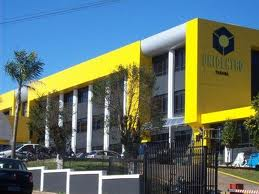
\includegraphics[scale=.5]{unicentro.jpeg}
      \label{fig:unicentro.jpeg}
      \caption{A nova Unicentro}
    \end{figure}
  \end{minted}

\end{frame}

%------------------------------------------------------------

\begin{frame}[fragile]
  \frametitle{Figuras}


    \begin{figure}
      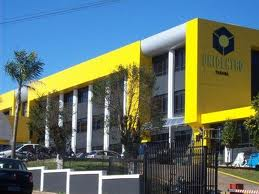
\includegraphics[scale=.5]{unicentro.jpeg}
      \label{fig:unicentro.jpeg}
      \caption{A nova Unicentro}
    \end{figure}

\end{frame}

\section{Temas}
\subsection{Mudando a aparência da apresentação}
%------------------------------------------------------------

\begin{frame}
  \frametitle{Temas}
  Os temas mudam o \textit{look and feel} da sua apresentação. \\

  Para mudar seu tema utilize o comando no preâmbulo do documento root : \newline \newline
  \textcolor{red}{$\backslash$usetheme\{Warsaw\}}
  \\
  Os temas disponíveis são os seguintes:
  \newline
  \newline

  \begin{tabular}{cccc}
      Antibes     &  Bergen       &  Darmstadt   &   Ilmenau  \\
      Boadilla    &  Copenhagen   &  Hannover    &   Marburg \\
      Frankfurt   &  Goettingen   &  Malmoe      &   Rochester \\
      Juanlespins &  Madrid       &  Pittsburgh   \\
      Montpellier &  Paloalto     &  Berlin       \\
      Singapore   &  Berkeley     &  Dresden      \\
  \end{tabular}
\end{frame}

%------------------------------------------------------------

\begin{frame}
  \frametitle{Cor dos temas}

  \begin{itemize}[<+->]
     \item Ainda é possível especificar a cor do tema escolhido.
     \item Para isso, usamos o comando $\backslash$usecolortheme\{color\}
     \item As cores disponíveis são:
        \begin{tabular}{cccc}
          albatross & crane & beet & dove \\
          fly & seagull & wolverine & beaver\\
        \end{tabular}
  \end{itemize}

\end{frame}

\section{Transições}
\subsection{Efeitos nos slides}
%------------------------------------------------------------

\begin{frame}[fragile]
  \frametitle{Transições de Slides}

  \begin{itemize}
     \item Com o Beamer também é possível definir efeitos transições de slides.
     \item Porém, diferentes visualizadores de pdf podem interpretar de diferentes maneiras os efeitos.
  \end{itemize}

  \begin{block}{Exemplo:}
    \begin{minted}[fontsize=\scriptsize]{tex}
        \begin{frame}
          \frametitle{Examplo Boxin }
          \transboxin
          Corpo do frame
        \end{frame}
    \end{minted}
  \end{block}

\end{frame}

%------------------------------------------------------------
\begin{frame}[fragile]
  \transboxin

  \begin{block}{Exemplo 2:}
    \begin{minted}[fontsize=\scriptsize]{tex}
        \begin{frame}
          \frametitle{Examplo blinds Horizontal }
          \transblindshorizontal[duration=2, direction=25]
          Corpo do frame
        \end{frame}
    \end{minted}
  \end{block}
\end{frame}

%-------------------------------------------------------

\begin{frame}[fragile]
  \transblindshorizontal[duration=2, direction=25]

  \begin{block}{Alguns opções de transições}
      \centering
      \begin{tabular}{l}
        $\backslash$transblindshorizontal \\
        $\backslash$transblindsvertical   \\
        $\backslash$transboxin \\
        $\backslash$transboxout \\
        $\backslash$transdissolve \\
        $\backslash$transglitter \\
        $\backslash$transslipverticalin \\
        $\backslash$transslipverticalout \\
        $\backslash$transhorizontalin \\
        $\backslash$transhorizontalout \\
        $\backslash$transwipe \\
        $\backslash$transduration\{2\} \\
      \end{tabular}
  \end{block}
\end{frame}

\begin{frame}
  \begin{center}
    Obrigado!!
  \end{center}

  \begin{block}{}
    \begin{center}
      Mais Inforamções sobre Beamer acesse o site: \\
      {\scriptsize
      \hyperref[http://www.ctan.org/tex-archive/macros/latex/contrib/beamer/doc/]{http://www.ctan.org/tex-archive/macros/latex/contrib/beamer/doc/}}
    \end{center}
 \end{block}

\end{frame}


\end{document}


